\subsection{Ola Language Compiler Frontend}

This section introduces the key components and functionalities of the Ola language compiler frontend. We will discuss the process of lexical analysis, syntax parsing, Abstract Syntax Tree (AST) generation, semantic analysis, and LLVM Intermediate Representation (IR) generation in detail.

The processing flow of the compiler frontend is shown in the following figure\ref{fig:ola-lang-compiler-frontend}:

\begin{figure}[!ht]
    \centering
    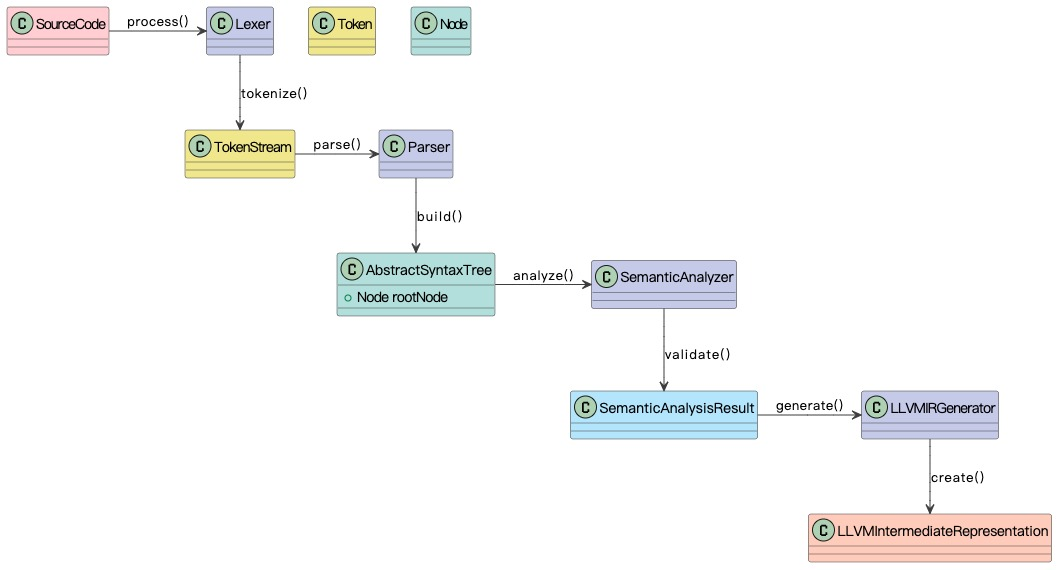
\includegraphics[width=0.8\textwidth]{ola-lang-compiler-frontend.jpg}
    \caption{Ola-lang Compiler Frontend}
    \label{fig:ola-lang-compiler-frontend}
\end{figure}



\subsubsection{Ola Language Parser}
\subsubsection*{Lexical Analysis}
Lexical analysis is the first stage of the compiler front-end. In this phase, the goal is to break down the source code into a series of tokens. The Ola language lexer will handle the following elements:
\begin{itemize}
\item Keywords
\item Identifiers
\item Operators
\item Literals (such as strings, numbers, and boolean values)
\item Comments
\item Delimiters (such as parentheses and commas)
\end{itemize}
Additionally, the lexer will eliminate whitespace and comments, ensuring a clean token stream for the next stage.

\subsubsection*{Syntax Parsing}
Syntax parsing is the process of transforming the tokens generated in the lexical analysis phase into an Abstract Syntax Tree (AST). The Ola language compiler will implement a top-down parser, such as a Recursive Descent Parser, to support Ola language's grammar.

This section will also discuss the implementation of error handling and recovery mechanisms, ensuring that the parser can handle syntax errors gracefully and provide helpful error messages to the user.

\subsubsection*{Abstract Syntax Tree (AST) Generation}
During the syntax parsing phase, the parser will generate an AST representing the program's structure. This section will explain the design of the AST data structures and the process of constructing the AST during parsing. Additionally, it will cover the benefits of using an AST, such as enabling easier manipulation and analysis of the code's structure.

The Ola compiler seamlessly integrates the Lexical Analysis, Syntax Parsing, and Abstract Syntax Tree (AST) Generation processes, forming a cohesive and efficient pipeline. By leveraging the LALRPOP framework, these stages work in harmony, transforming the Ola source code into an AST representation that is suitable for subsequent compiler phases. This unified approach not only simplifies the implementation but also enhances the performance and robustness of the Ola compiler.

By following these steps, the compiler can efficiently convert the Ola source code text into a sequence of tokens:

\begin{itemize}

  \item The first step in implementing the lexical analysis phase of the Ola compiler is to define lexer rules for various token categories, including keywords, identifiers, literals, and operators. These rules should be based on the provided EBNF grammar rules. We created a file named Ola.lalrpop that describes Ola's EBNF grammar rules.

  \item After defining the lexer rules, the next step is to integrate the lexer with the parser. This can be achieved by using the \texttt{lexer} attribute in LALRPOP grammar rules. The \texttt{lexer} attribute specifies which lexer rule should be used to recognize a particular grammar production.

  \item Ola compiler provides error handling and reporting. If the lexer encounters an unexpected character or a malformed token, it generates an error with the corresponding position in the input text. This information can be used to provide helpful error messages to the user.

\end{itemize}

Once the lexical analysis phase is complete, the generated sequence of tokens can be passed to the parser, which will construct an abstract syntax tree (AST) based on the defined grammar rules. This AST can then be further processed by subsequent phases of the Ola compiler, such as semantic analysis, optimization, and code generation, ultimately producing executable code for the target platform.

By leveraging the powerful LALRPOP framework, the Ola compiler can efficiently perform lexical analysis and provide robust error handling, ensuring that the compiler is user-friendly and capable of handling complex Ola source code.

\subsubsection{Semantic Analysis}

The Semantic Analysis phase of the Ola compiler is an extensive process that ensures the program's correctness and consistency. As previously mentioned, this phase consists of several sub-tasks. Here, we delve deeper into each sub-task, providing a more detailed and comprehensive explanation of the process.

\subsubsection*{Symbol Resolution}

The compiler analyzes the program's scope and context to resolve symbols accurately. It distinguishes between local and global variables, function declarations, and type definitions. The symbol table, which holds information about each symbol, is updated as the compiler traverses the AST. During this process, the compiler also checks for naming conflicts and multiple declarations, ensuring that the program adheres to Ola's scoping rules.

\subsubsection*{LibFunction Identification}

In the semantic analysis phase, we will identify all libFunction names that users call. We will also construct prototype code for these LibFunctions and verify whether the parameters used to call them match the parameter types and numbers in the prototype code. If there is a match, we will record them for easy processing of IR generation for Lib Functions in subsequent LLVM IR generation phases.

\subsubsection*{Type Checking}

The compiler ensures that each operation and expression in the program involves operands of compatible types. In this stage, the compiler also infers the types of expressions when necessary and enforces type constraints for function calls, assignments, and arithmetic operations.

\subsubsection*{Control Flow Analysis}

In addition to checking for unreachable code and infinite loops, the control flow analysis process verifies that:

\begin{itemize}
 \item All code paths in a function that should return a value must end with a return statement.
 \item Break and continue statements appear only within loops.
 \item Variables are declared before they are used.
\end{itemize}

\subsubsection*{Constant Expression Evaluation}

During this step, the compiler performs the following tasks:

\begin{itemize}
  \item Evaluates arithmetic and bitwise operations on constant expressions at compile-time, ensuring that the generated code is more efficient.

  \item Detects potential errors, such as array index out-of-bounds, by evaluating expressions that involve constants.

  \item Folds constant expressions, such as mathematical operations or string concatenations, reducing the code size and improving execution efficiency.

\end{itemize}

\subsubsection*{Semantic Validation}
 The final step of the semantic analysis phase consists of several validation checks, including:

\begin{itemize}
  \item Verifying that variables are initialized before they are used.
  \item Ensuring that variables, functions, and types are declared only once within a given scope.
  \item Checking that all required function arguments are provided and that excess arguments are not supplied.
  \item Validating that return statements are used correctly within functions.

\end{itemize}

The Semantic Analysis phase is crucial for the robustness and correctness of the Ola compiler. By performing these comprehensive checks, the compiler can guarantee that the generated code adheres to the language's semantic rules and is free from errors that might lead to unexpected behavior during execution. With a semantically verified AST, the Ola compiler proceeds to the subsequent phases of the compilation process, ensuring the efficient translation of the source code into executable code tailored for the OlaVM.

\subsubsection{Generator: from richAST to LLVM IR}
